\documentclass[10pt]{article}
\usepackage[margin=0.7in]{geometry}
\usepackage{amsmath,amssymb,graphicx,booktabs,xcolor,hyperref}
\definecolor{ink}{HTML}{253C59}
\hypersetup{colorlinks=true,urlcolor=ink,linkcolor=ink}
\setlength{\parindent}{0pt}\setlength{\parskip}{6pt}\setlength{\emergencystretch}{2em}
\begin{document}
{\Large\bfseries\color{ink} Target-dependent torus multiplier fibre}\par
{\small 24 November 2026 \quad Proposed mechanism; recovery gate precedes scaling}

\textbf{Written construction.} Fix relative raw labels and solve for a common
torus multiplier from the public target. Two leaves give a proposed univariate
degree bound8; six leaves give384 per branch. These bounds are independent
of $q,K$ because the multiplier---and therefore the base---is free. This
component supplies no native/formal qualification, solver implementation,
experiment, discovered root or cost/exponent result. [pcc:unverified]

\textbf{Original family.} Keep $p=2^{255}-19$, $A=486662$, $a=60824497$,
$q=213156431$, $K=20633$, original $h$ of order $aq$ and
$S=\{h^{j+at}:1\le j\le K,0\le t<q\}$. A candidate output belongs to
$S_\sigma=\sigma S$, which need not be the original unshifted base.

\textbf{Cayley chart.} With $\alpha_i=(a_i,b_i)$ in the norm-one torus,
\begin{align*}
\sigma(c)&=\frac{1+c\sqrt2}{1-c\sqrt2}
 =\frac{1+2c^2+2c\sqrt2}{1-2c^2},\\
V&=1-2c^2,\qquad U_i=a_i(1+2c^2)+4b_ic,\\
N_i&=A(\epsilon_iV-U_i),\quad D_i=2U_i,\quad u_i=N_i/D_i,
\qquad \epsilon_i\in\{1,-1\}.
\end{align*}
Each $N_i,D_i$ has degree at most2. Retain the $V,U_i$ guards and the
projective point $c=\infty$, $\sigma=-1$. Canonicality/norm, rational
ordinates and nonidentity eightfold images remain separate checks.

\textbf{Two-leaf numerator.} For finite raw target $R=(r,s)$, Montgomery
$f_3(x,y,r)=(x-y)^2r^2-2((x+y)(xy+1)+2Axy)r+(xy-1)^2$.
Writing $Z=D_1D_2$, clear $D_1^2D_2^2$:
\begin{align*}
P(c)={}&(N_1D_2-N_2D_1)^2r^2\\
 &-2\big((N_1D_2+N_2D_1)(N_1N_2+Z)+2AN_1N_2Z\big)r\\
 &+(N_1N_2-Z)^2.
\end{align*}
The written bound is $\deg_cP\le8$, four branch choices. It still needs
coefficient/identity and lifting qualification. Zero polynomials are
degenerate families; caps/unsupported extraction are incomplete outcomes.
Roots require rational sign lifts and exact group/target replay, not just
the summation equation. [pcc:unverified]

\textbf{Public target and six leaves.} The API receives public spec/templates,
$R/Q$ and limits, no known multiplier/candidate list/scalar/section. For
nonidentity prime-group $Q$, $R=[8^{-1}\bmod\ell]Q$ is public; all8 torsion
translates are required for complete cofactor-sector coverage. An identity
target needs its own exact branch. The per-variable Semaev bound gives
$\deg_cP\le m2^m$, hence384 for $m=6$. Polynomial construction/factoring,
all64 branch choices/sectors and filtering are still actual work. The current
unshifted Circuit is not a shifted-map fidelity theorem. [pcc:unverified]

\newpage
{\large\bfseries\color{ink} The shared-base gate and prospective tests}\par
\begin{center}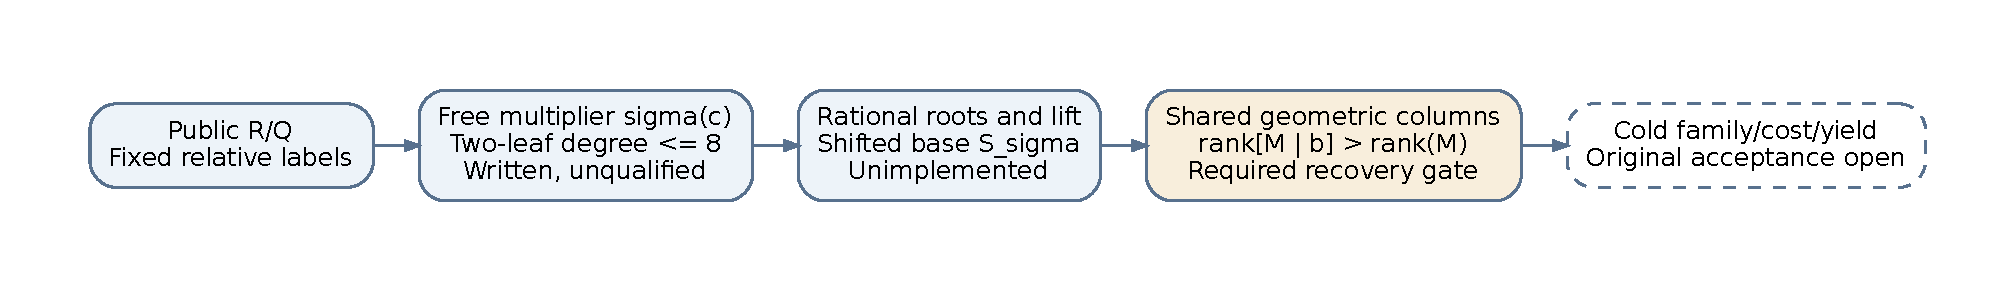
\includegraphics[width=\linewidth,height=1.35in,keepaspectratio]{diagram.pdf}\end{center}

\textbf{Parameter stabilizer.} $H_q=\langle h^a\rangle$ permutes the root
index. Under exact order and interval bounds it is the entire stabilizer of
the raw parameter set: a stabilizer lies in $\langle h\rangle$, then preserves
$J=\{1,\ldots,K\}$ modulo $a$; its singleton cyclic boundary forces zero
shift. There are $(p+1)/q$ parameter-base classes. Geometric/cofactor aliases
still need separate canonicalization. Relabelling a point is not a new row.
[pcc:unverified]

\textbf{Linear recovery discriminator.} After charging known-log columns and
canonicalizing actual geometric images, write
\[
Mz=a+bx,\qquad Q=xG.
\]
From these linear data alone, a useful witness satisfies
\[
v^TM=0,\quad v^Tb\ne0,\quad
x=-\frac{v^Ta}{v^Tb};\qquad
\operatorname{rank}[M\mid b]>\operatorname{rank}M.
\]
Private columns force full row rank and no left-kernel recovery. A common
base-class match is not enough. New overlap or logarithm-transport structure
must be demonstrated with costed actual rows/tags; the torus encoding is not
assumed to be a group homomorphism. [pcc:unverified]

\textbf{Proposed order of work.} First qualify the guarded two-leaf compiler
and native polynomial/identity checks. Then use the public-target-only root
interface on the fixed toy $p=101,A=95,h=(17,12),a=17,q=3,k=8$, templates
$h,h^2$; compare all102 torus multipliers including infinity and supported
raw targets against direct group enumeration. Original-field public $u=9$
and its negative, plus one known-consistent validation target, retain original
$q,K$. A known multiplier never enters the query. Unsupported, zero-polynomial,
alias/inverse, malformed and forced-cap controls remain explicit.

Before six-leaf scaling, freeze a common-base/column-sharing method and test
actual $M,a,b$ with exact ranks and a held-out scalar replay. No larger
backend/campaign is justified by the degree bound alone. PROTOCOL.md is
prospective and schedules no experiment or paid job. [pcc:unverified]

\textbf{Exponent gate.} Only under the separate COMMON-base assumptions
yield $B^6/\ell$, decomposition $B^\gamma$ and useful row rank, balancing
$\ell B^{\gamma-5}$ with $B^2$ gives $2/(7-\gamma)$. The free-multiplier
fibre establishes neither that yield nor $\gamma$; inserting $\gamma=0$
would lose the private-base cost. All original family/setup/index/memory/
kernel/recovery criteria remain. [pcc:unverified]

\textbf{Secondary audit.} Independent sign flips may diagonalize the old
cover's quadratic pullback-degree form. This is a conditional classical-law
argument, with actual cover/maps/degrees still unconstructed here. It supplies
no solver and does not promote the frozen energy draft. [pcc:unverified]

\textbf{Sources/status.} EFD Montgomery affine formulas; Yokoyama etal,
\href{https://nutmic2019.imj-prg.fr/confpapers/SemaevECDLP.pdf}{section2.1/Proposition1};
official FLINT factor/root interface; Milne AV Corollaries5.3/5.4;
Farashahi etal Theorem3 with unramified-cover hypothesis. KB wrapper127,
original Semaev PDF403, no novelty clearance. No measured graph or canonical
scoreboard change: only a proposed mechanism and discrimination protocol.
\end{document}
